\newpage
\section{Results in the reporting period}
% [max 3 pages including figures]

%(interim highlights)  \\
%A short paragraph (e.g. 200-300 characters) for presenting the interim results in the global picture. Details of the interim results (e.g. highlights about specific methodology or specific results) 

\subsection{Toward More Intuitive Teleoperation Interfaces}
The first results reported in this document regard the exploration of intuitive interfaces for teleoperation architectures. Indeed, the concept of TelePhysicalOperation has been proposed [J.1], to control the teleoperated robot using a \enquote{Marionette} type of interface. This kind of teleoperation emerges from the blending of the classical teleoperation used to control a remote robot, and the physical human robot interaction used to control a remote or a collaborative robot (\figurename~\ref{fig:tposcheme}). 

\begin{figure}[H]
	\centering
	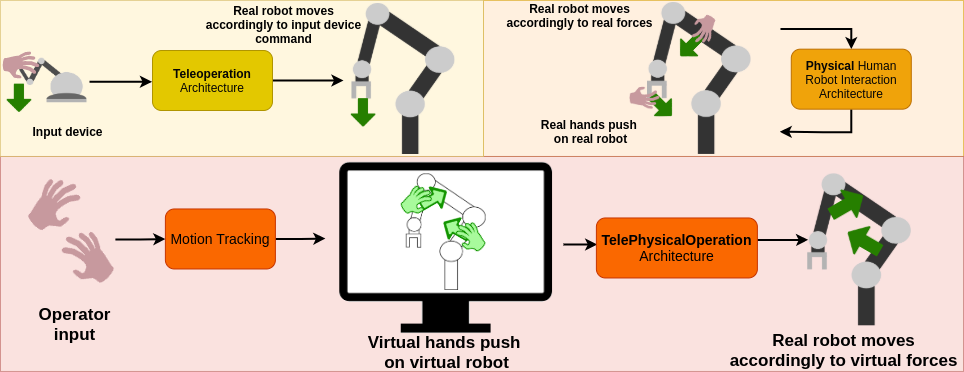
\includegraphics[width=0.85\linewidth]{img/TPOScheme}
	\caption{Concept of TelePhysicalOperation. Above, schematics of the traditional teleoperation and the physical human robot interaction interfaces. Below, the scheme of TelePhysicalOperation, derived by the combination of the two above controlling interfaces}
	\label{fig:tposcheme}
\end{figure}

By selecting specific control points on the robot kinematic chains, the operator can apply virtual forces that in a remote manner resembles the real applied forces of a physical human robot interaction exploited to guide the robot during a teaching/collaborative task. Thus, the proposed method permits to command the robot keeping a safe distance but also exploring the intuitiveness of the physical interaction. 
%
%\begin{figure}[H]
%	\centering
%	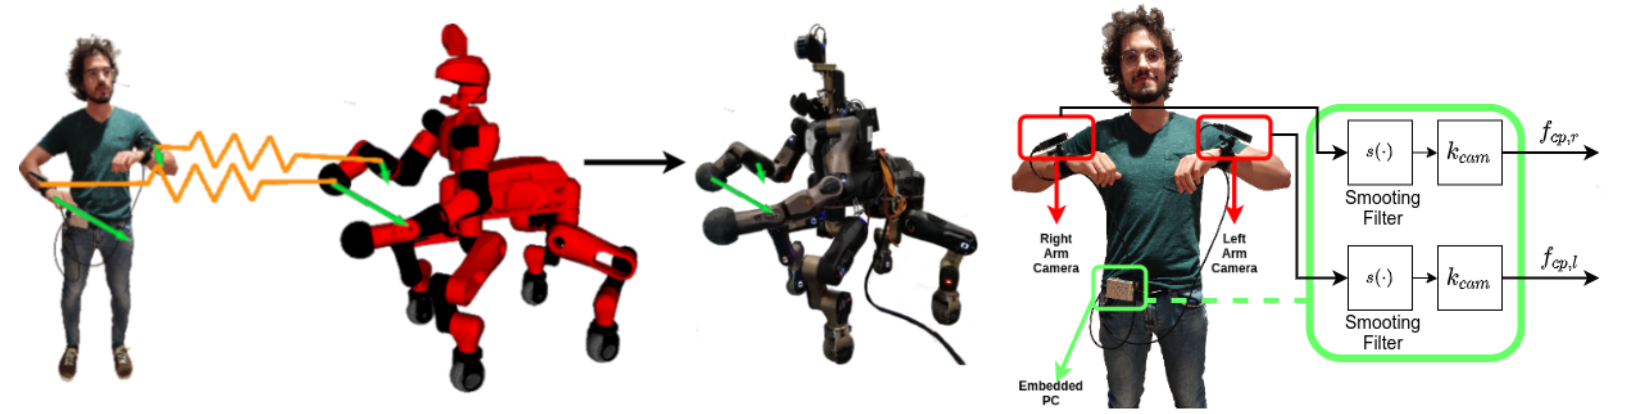
\includegraphics[width=0.9\linewidth]{img/TPOConcept}
%	\caption{On the right, the TelePhysicalOperation concept follows a \enquote{Marionette} type interaction: the operator generates virtual forces that can be selectively applied on specific locations on the robot segments. On the left, the TPO suit, the motion tracking interface used to gather operator arm movements and generate virtual forces $\boldsymbol{f}_{cp}$. }
%	\label{fig:tpoconcept}
%\end{figure}
%
The virtual forces are applied along the kinematic chain of the robot, which responds regulating its motion to comply with them as in a compliant physical human-robot interaction. The virtual forces are generated by virtual springs which link the arms of the human operator and the selected robot body parts, resembling a \enquote{Marionette} motion generation interface. The interface allows to virtually interact with the robot arms, hence controlling the robot manipulation ability, or with the body, hence controlling the robot mobility ability.
%
The virtual forces are generated through the motion of the operator arms. To track such motions, we make use of a lightweight and low-cost motion capture solution based on Visual-Simultaneous and Localization Mapping (V-SLAM) tracking cameras, worn on the operator wrists. In such a way, the movements of the user arms are associated with the elongation of the virtual spring used to compute the final virtual force that will be applied to the selected robot body part.

We conducted a series of experiment with the CENTAURO~\cite{Centauro2} robot [J.1]. For example, in \figurename~\ref{fig:tpoexp}, with the application of two virtual forces on two different points of the same arm of the robot, the operator can first activate the shoulder and the elbow joints to go over the obstacles (first image) and then bend the wrist to reach the button to be pressed from above (second and third images).   

\begin{figure}[H]
	\centering
	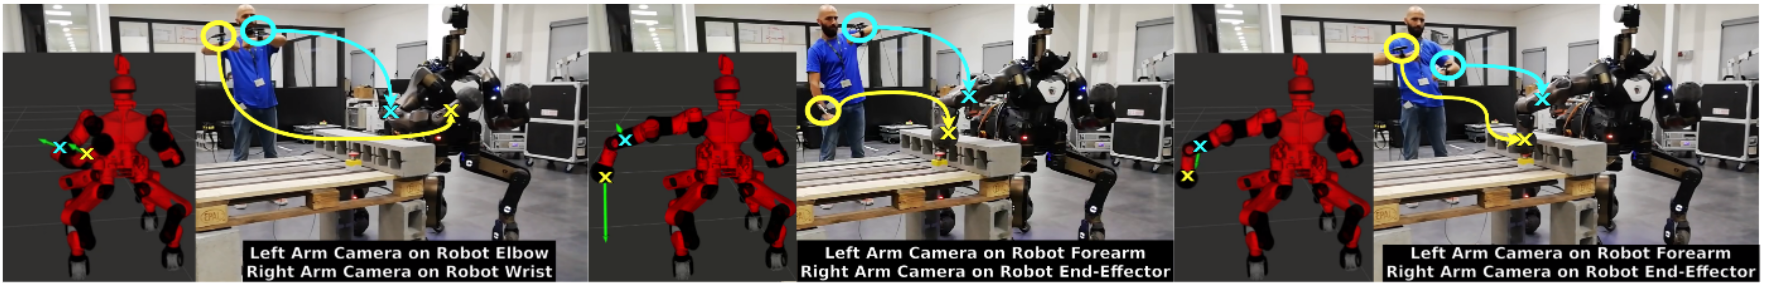
\includegraphics[width=0.95\linewidth]{img/tpoExp}
	\caption{In this experiment the goal is to press a button obstructed by some bricks. The cyan and yellow marks indicate where the virtual forces are applied by the operator. The robot visualization (RViz) shows the input directions commanded by the user (green arrows).}
	\label{fig:tpoexp}
\end{figure}


\subsection{Enhancing the Teleoperation Interfaces}
One common challenge with mobile manipulators is that both the robot arm(s) and the mobile platform must be considered when performing a locomanipulation tasks. Indeed, a change of control mode (from arm to mobile base and vice versa) is necessary each time the operator wants to move the mobile base or the arm, an operation that is repetitive and may increase the operator effort and the task execution time. As an alternative more input interfaces to control at the same time the base and the arm may be exploited, but this may augment the operator burden. To face this challenge, it is necessary to provide the robot with more autonomy, for example with whole-body controllers or other kind of techniques to switch automatically the control mode.
To address this problem, we have proposed a shared control interface for locomanipulation tasks to automatically generate mobile base motions even when only the arm is commanded [C.3]. In such a way, the operator can control exclusively the arm, without taking care of changing the control modality from the arm to the mobile base, and without taking care of the limited workspace of the arm. The proposed interface, integrated in the TelePhysicalOperation architecture, considers the manipulability level of the arm~\cite{Yoshi1985}, a measure strictly related to the kinematic singularities of the limb. If the robotic arm reaches a workspace region in which the manipulability in the direction of the applied virtual force is low, the generated motion is gradually switched to the mobile base. This permits to reach the desired end-effector goal without the necessity of switching from arm control to mobile base control, and assuring that the manipulability does not decrease beyond a defined threshold. 

In some scenarios, other autonomy features are necessary to accomplish successfully a task. In [C.3], [C.4] the mentioned manipulability-aware shared locomanipulation teleoperation has been enhanced with a strategy to regulate automatically the grasping forces on a object bi-manually transported by the robot \figurename~\ref{fig:tpoexpbox}.
In this way, the user is required to only command the object velocities (generating virtual forces from his/her arm movements), without worrying about arms manipulability, about switching from arms control to locomotion control, and about the grasping forces necessary to transport the load without dropping or damaging it.

\begin{figure}[H]
	\centering
	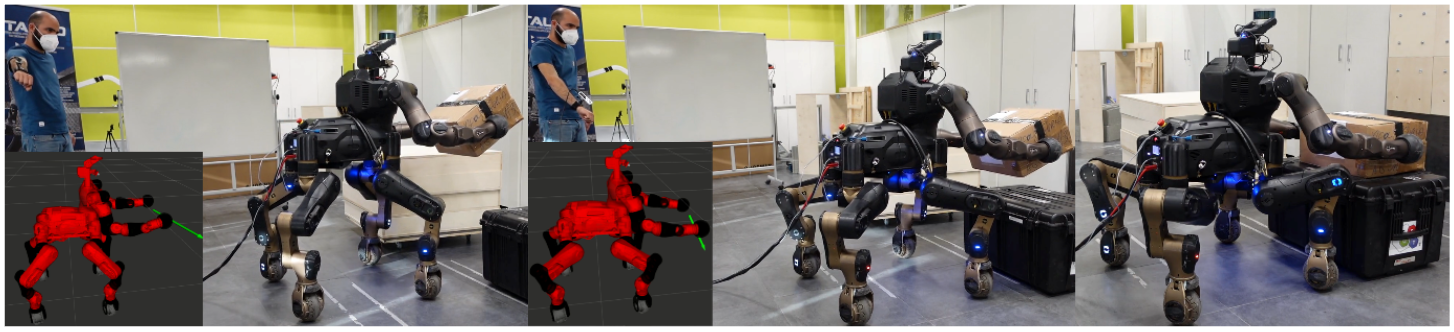
\includegraphics[width=0.9\linewidth]{img/tpoexpbox}
	\caption{The robot is teleoperated to transport the load to a location. The manipulability-aware shared locomotion is combined with a bimanual grasping feature to autonomously regulate the grasping forces applied on the object while accepting the operator commanded object velocities (shown as the green arrows in the robot visualization).}
	\label{fig:tpoexpbox}
\end{figure}

In parallel, haptic feedback have been explored [C.8]. Indeed, certain types of information about the status of the robot or of the task can not been transmitted to the user through a monitor or by watching directly the robot. To address the challenge, and further improve the TelePhysicalOperation paradigm, we have developed a sensorimotor interface~\cite{prattichizzo2021human} and integrated it into the TPO suit. In particular, the user wears two rings and two armbands, which can deliver vibration and skin indentation stimuli. 
The rings are also endowed with two small push buttons, providing additional input possibilities that, in the previous TPO works, had required the presence of an additional operator. Skin indentation stimuli are sent to the user to increase his/her awareness of the control command delivered to the robot and of the robot-environment interaction, whereas vibrations are used as acknowledgments about the execution of the command associated with a button.
User study evaluation with naive users teleoperating the CENTAURO robot showed a positive outcome for the devices integrated in the interface, assessing only a slight increase in the complexity of the additional devices worn.


\subsection{Laser-based Visual Teleoperation}
In the direction of simplify the control of complex robots, another intuitive teleoperation interface has been explored, developing a visual servoing framework which permits to control a robot with a laser emitter [J.4, C.6, C.7]. By pointing the laser in the environment, the operator is able to command even highly articulated robots effortlessly and efficiently. 
The perception layer that tracks the laser spot implements a neural network solution, based on YOLO~\cite{yolov5}. This has resulted to be a much faster and robust solution compared to common computer vision techniques, permitting to promptly detect goal position changes. 

In the main work that exploit this interface [J.4], the robot behavior is built around a Behaviour Tree, a flexible and modular planning structure, easily adaptable to different robot and different tasks. The evaluation of such architecture has been validated on the CENTAURO robot in a series of tasks, for example in a pick-and-place mission combining the manipulation and the locomotion ability of the robot (\figurename~\ref{fig:pickAndPlacePhoto}).

\begin{figure}[H]
	\centering
	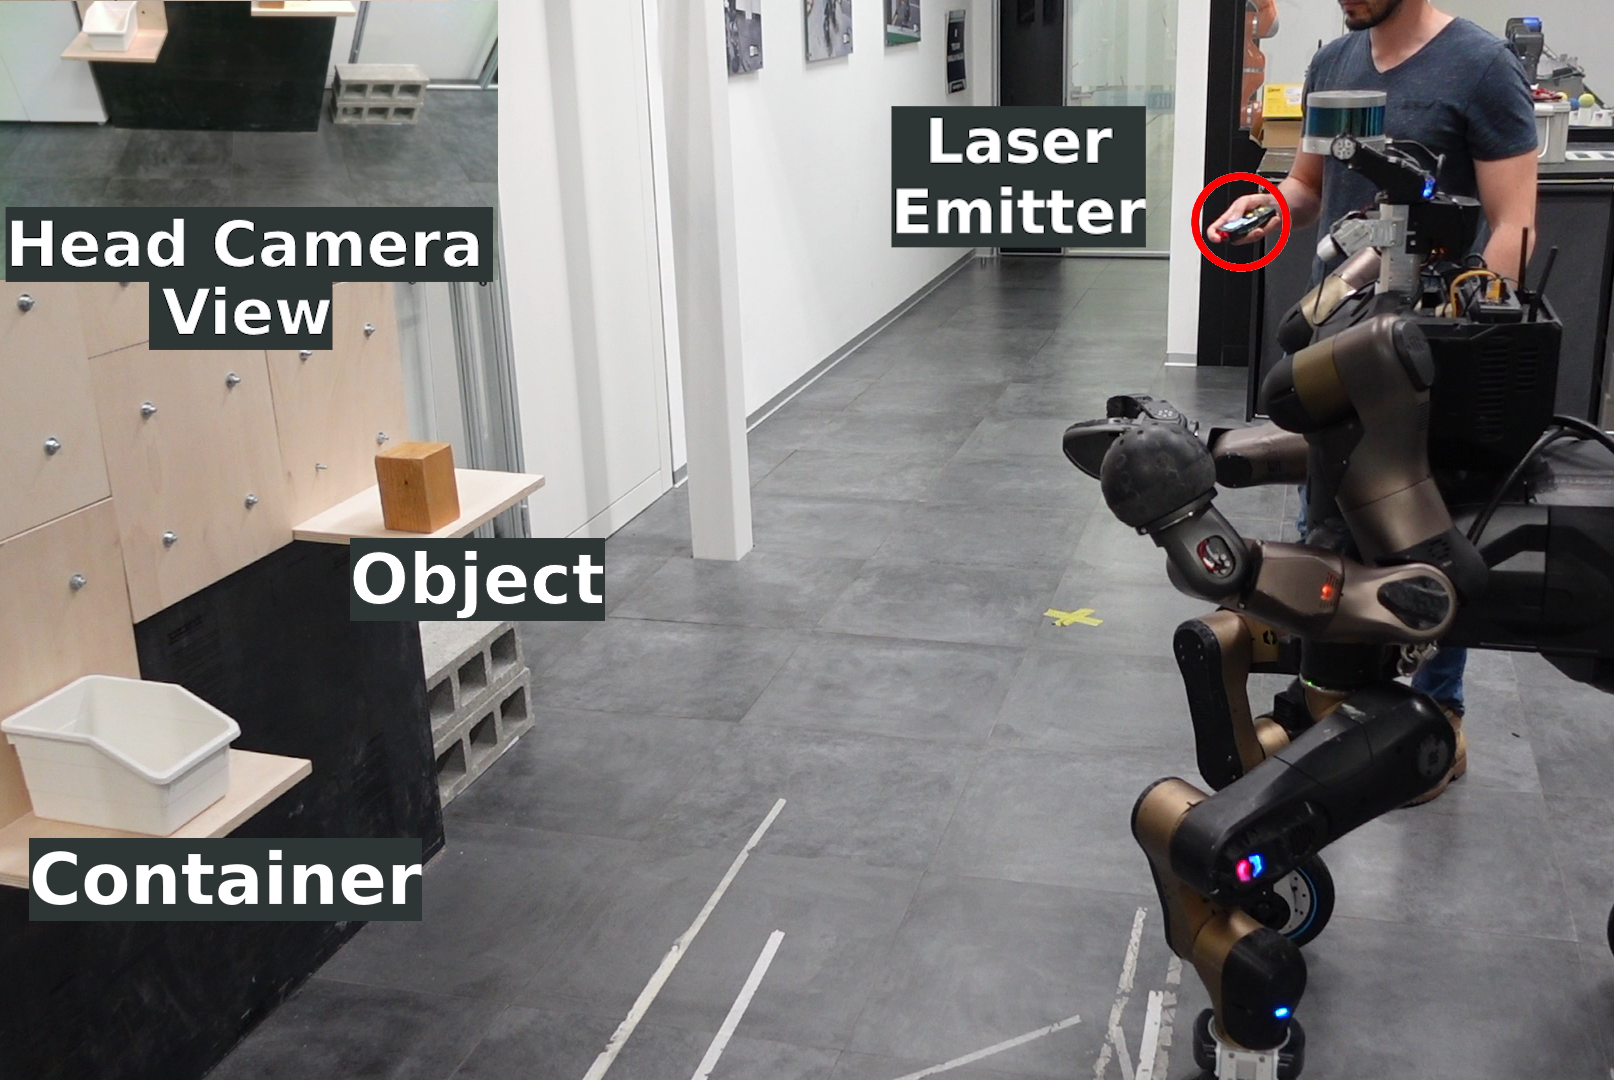
\includegraphics[height=0.2\linewidth, keepaspectratio]{img/grasp1Edited}
	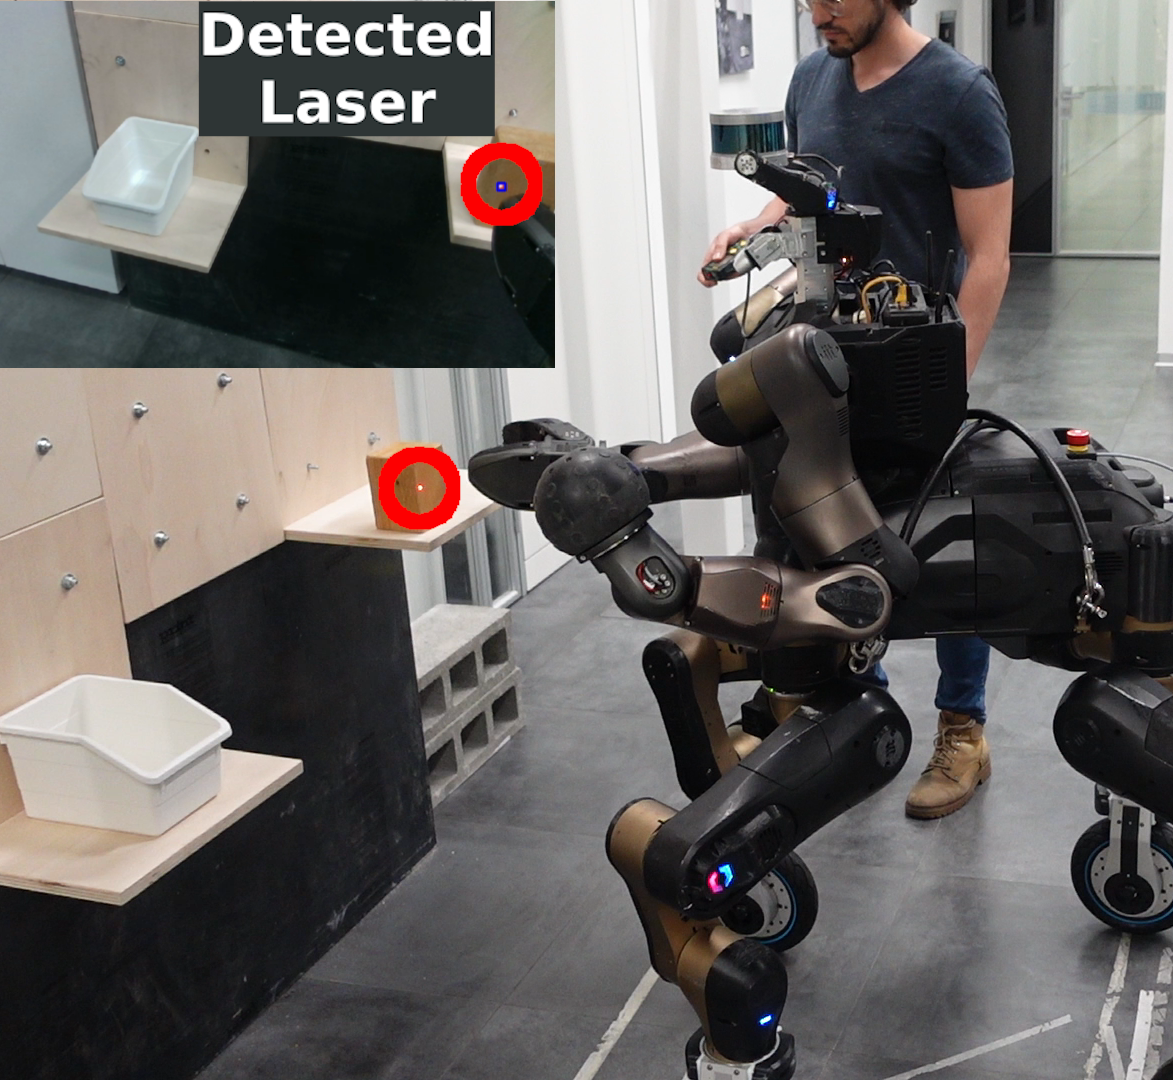
\includegraphics[height=0.2\linewidth, keepaspectratio]{img/grasp2Edited}	
	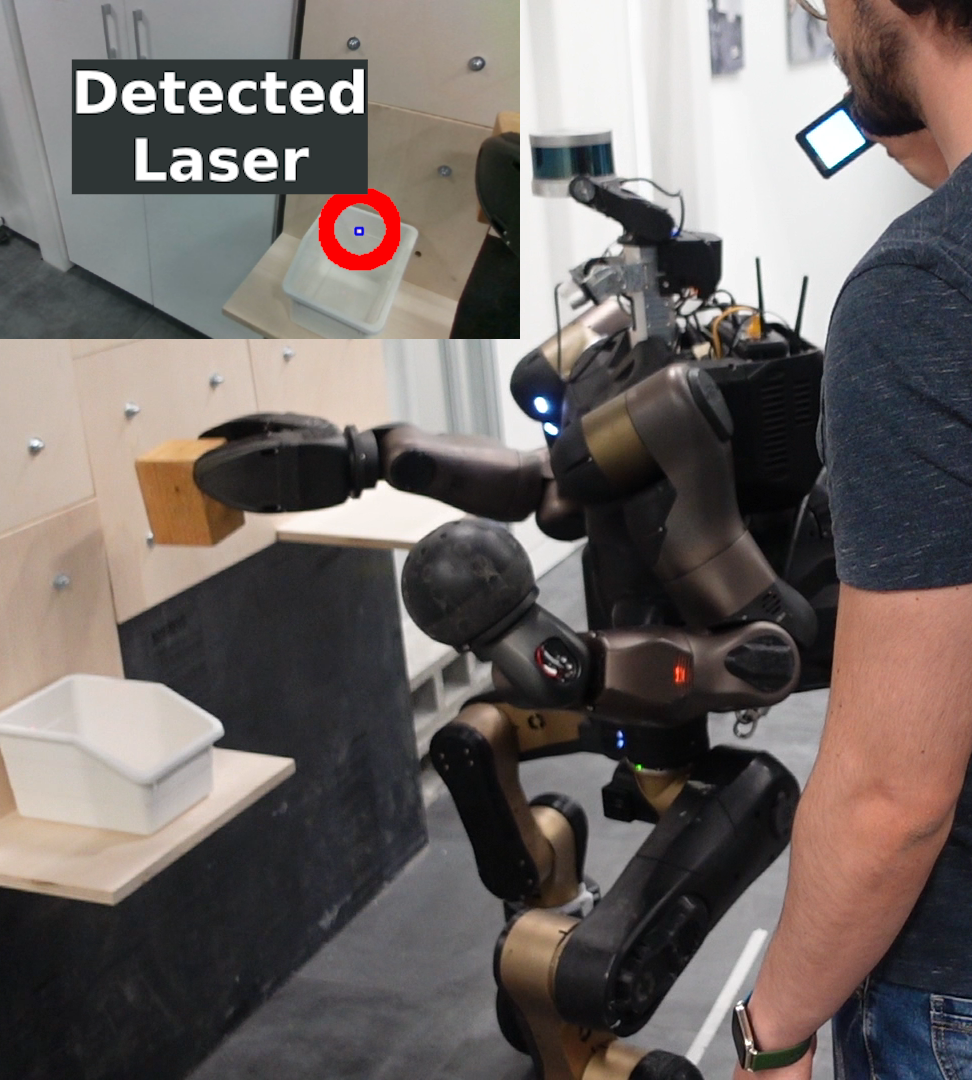
\includegraphics[height=0.2\linewidth, keepaspectratio]{img/grasp4Edited}
	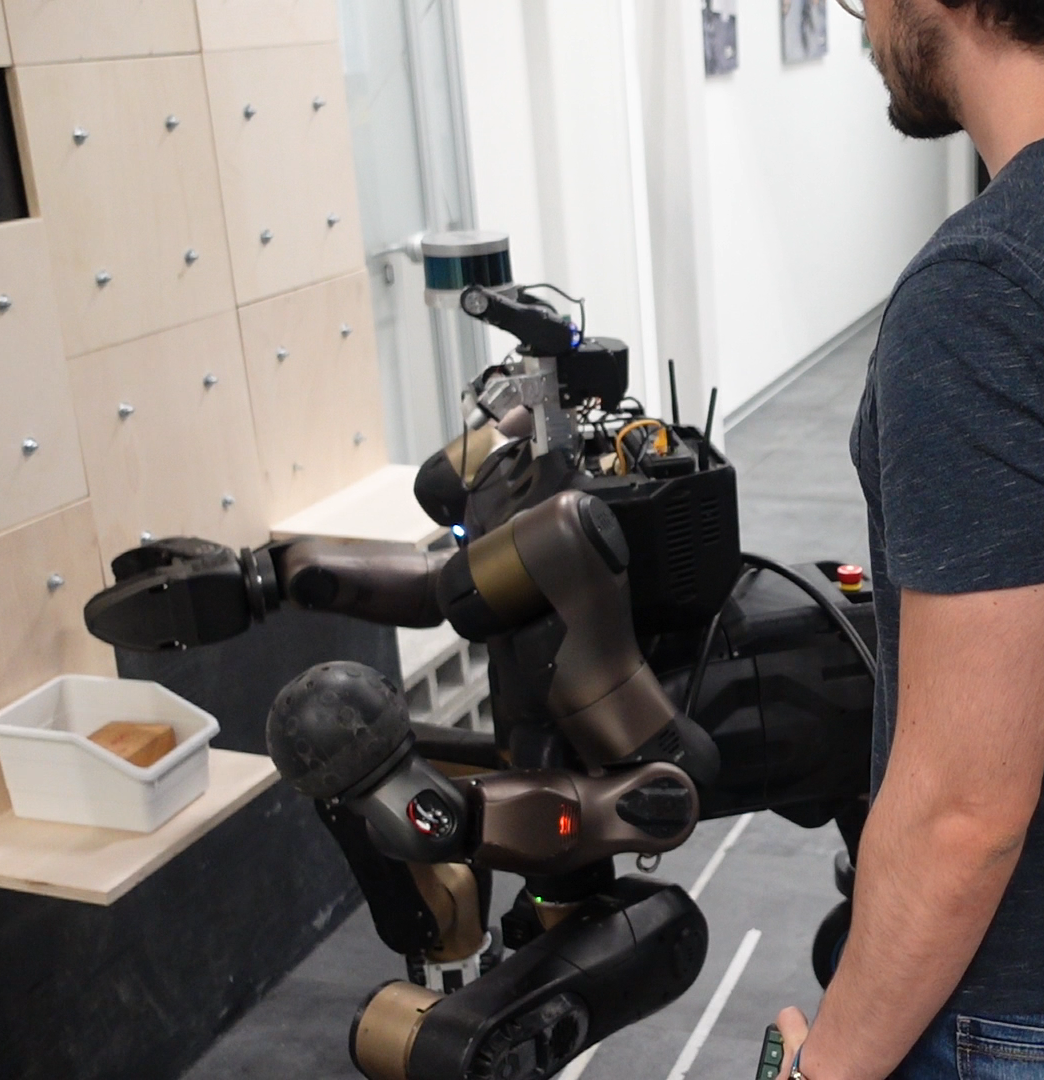
\includegraphics[height=0.2\linewidth, keepaspectratio]{img/grasp5Edited}
	\caption{Sequences of the pick-and-place experiment. The operator guides the robot toward the object, to place it into the container. Once the end-effector is in position, the user requests to grasp/release the object, interrupting temporarily the tracking of the laser.}
	\label{fig:pickAndPlacePhoto}	
\end{figure}

In other works [C.6 C.7], the laser-based teleoperation interface has been exploited for an assistive scenario. The target are impaired arm users, which have limited abilities on one or both arms, and need help for Activities of Daily Living (ADL). Hence, the laser is worn on the user's head permitting to command a fixed manipulator with head movements. Two control modalities are available, activated based on where the laser is pointed. 
When the laser is pointed onto the environment, the framework generates and executes a collision free trajectory toward the indicated goal. 
Instead, with the second modality, the user can \enquote{click} the keys of a paper keyboard by projecting the laser onto them. The keyboard permits to control the robot end-effector by commanding Cartesian velocities with a direction represented by the selected key. 

In \figurename~\ref{fig:pane3-frames}, it is reported an ADL task executed with the interface proposed, where the user, simulating an impairment on his right arm, commands the robot to hold the bread that must be cut.
In the leftmost image, it is shown how the user exploits the first modality to command the arm above the bread. In the second image, the user finalizes the robot end-effector position and close the gripper by projecting the laser on the keyboard.

\begin{figure}[H]
	\centering
 	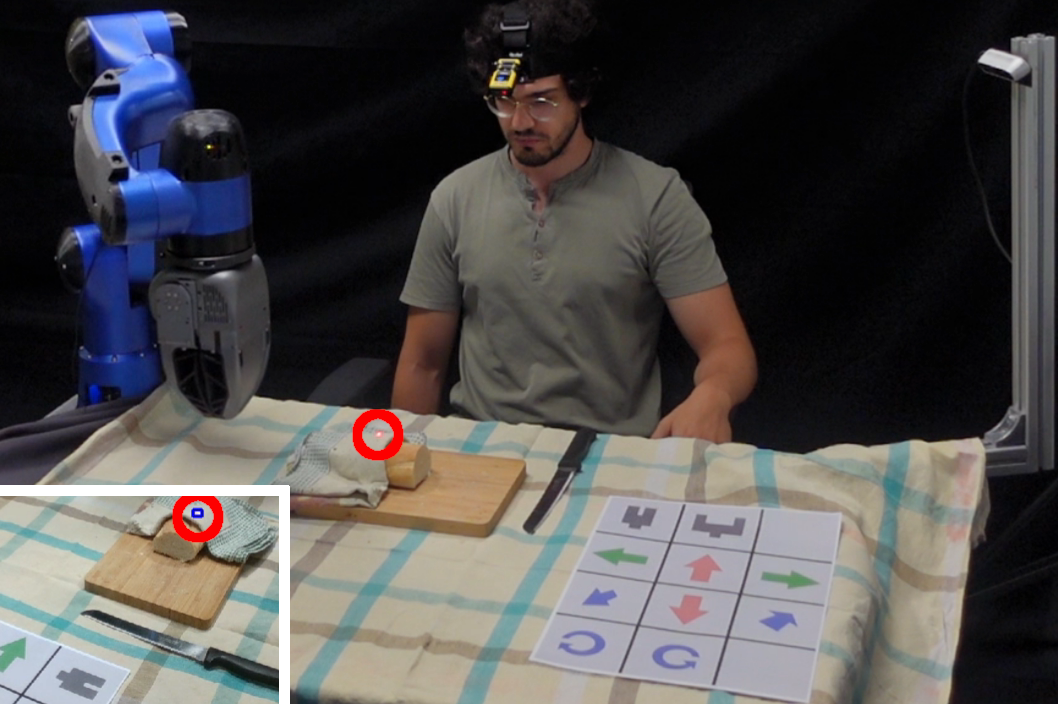
\includegraphics[width=0.22\linewidth]{img/pane-frame0edited.png}
	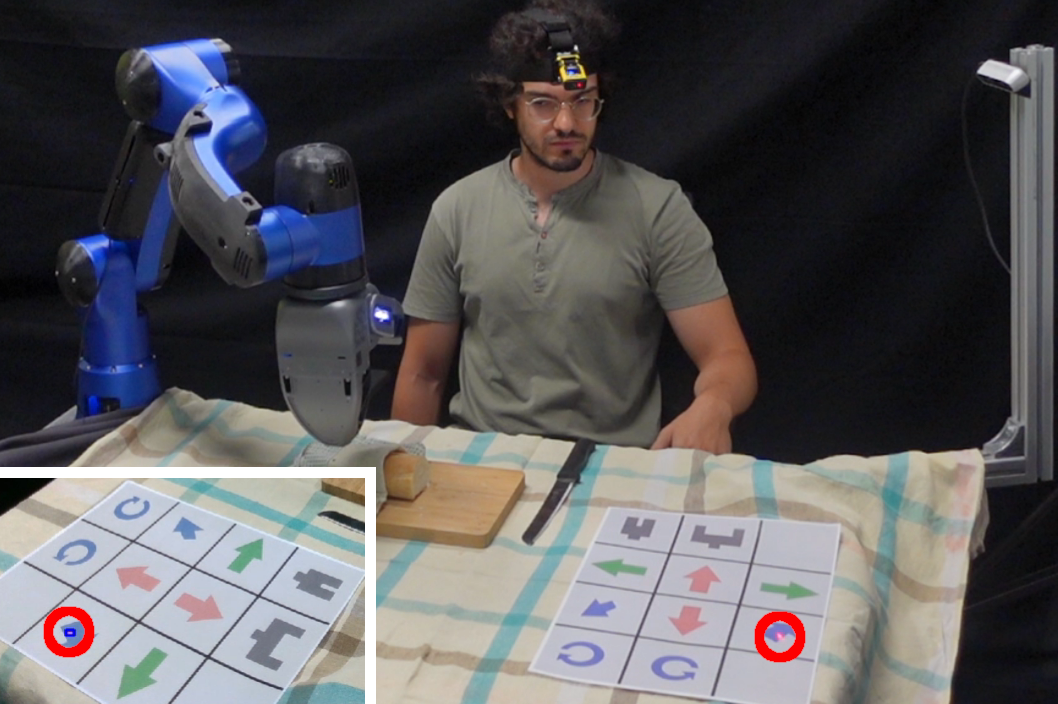
\includegraphics[width=0.22\linewidth]{img/pane-frame1edited.png}
	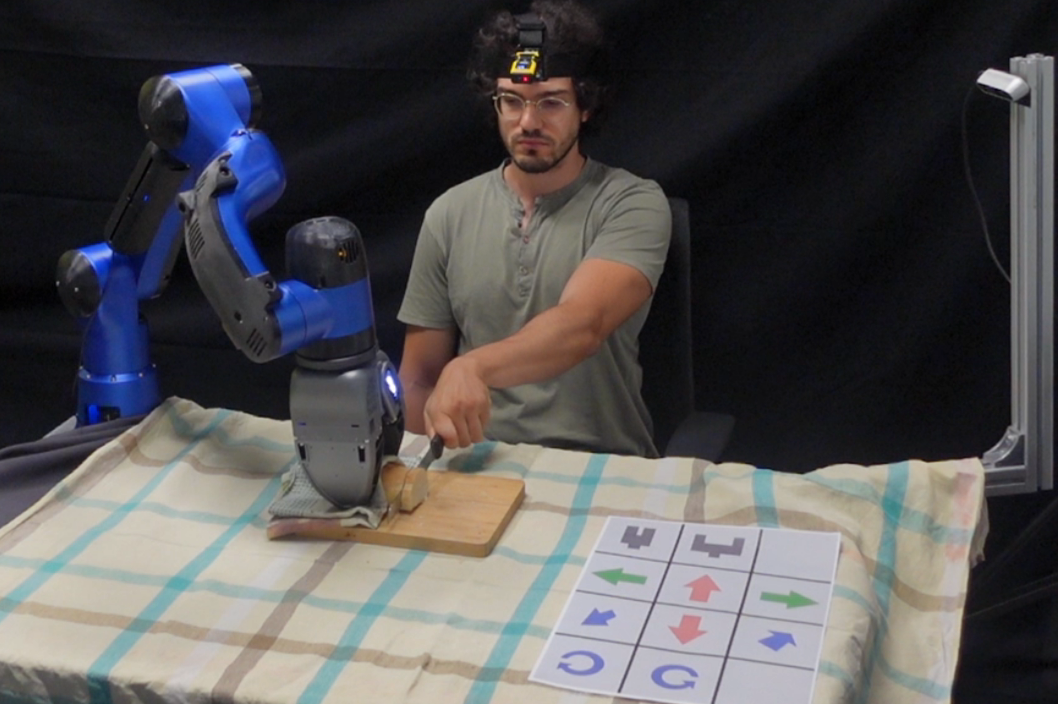
\includegraphics[width=0.22\linewidth]{img/pane-frame2edited.png}
	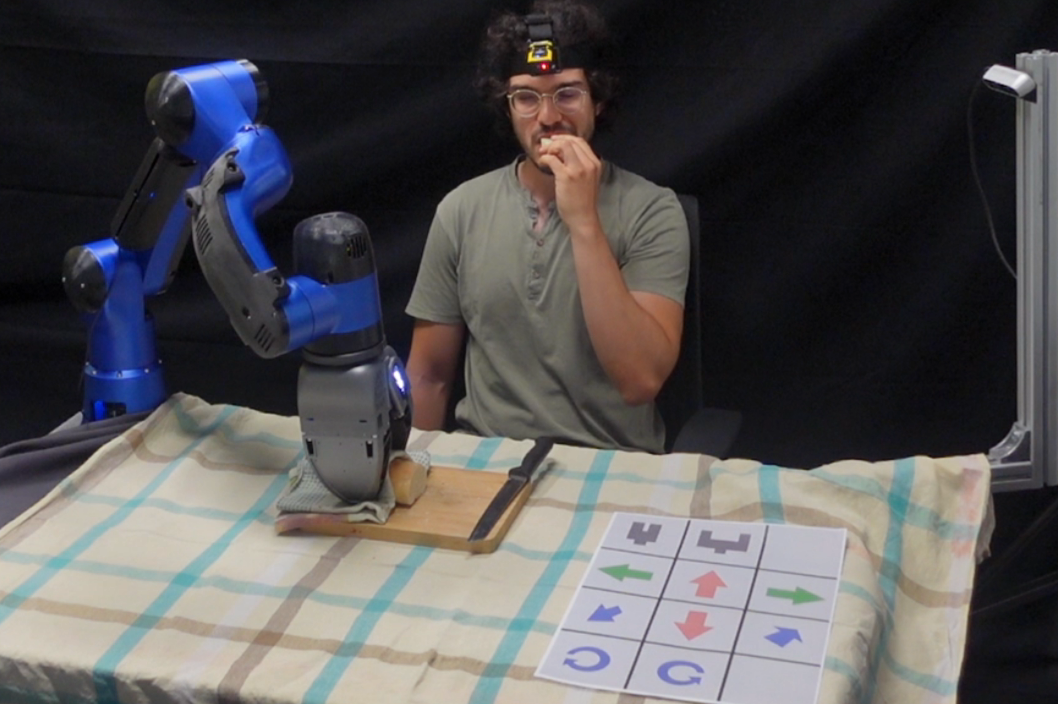
\includegraphics[width=0.22\linewidth]{img/pane-frame3edited.png}
	\caption{Sequences of the \enquote{cutting bread} experiment, with the camera view added in the frames when the robot is commanded, showing the detected laser spot.}
	\label{fig:pane3-frames}
\end{figure}

